\chapter{Use Cases}
\label{cha:useCases}

%----------
\section{Use Case Diagram}
\begin{figure}[H]
\begin{center}
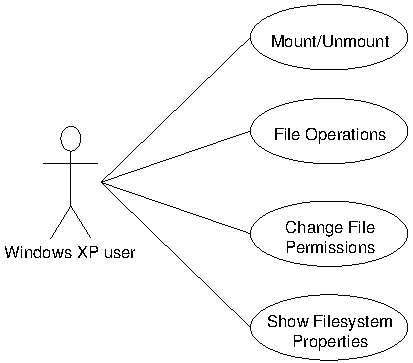
\includegraphics[width=8cm]{./files/inc/pic/useCaseDiagr}
\end{center}
\caption{\label{fig:useCaseDiagr}Use Case Diagram WinLFS}
\end{figure}

%----------
\section{Description}
Diagram \ref{fig:useCaseDiagr} shows all actions which an actor can take. All use cases are written in casual style, which describes use cases in an informal paragraph format. This style is more elaborate than the brief style, though less elaborate than fully dressed. It describes the main success scenario including possible errors an conditions. For WinLFS, this style seemed most accurate.
%\newpage

%----------
\section{Actors}
Windows XP users who use WinLFS file system driver to access their ext2 or ext3 partition for reading or writing.

%----------
\section{Use Case Descriptions}

\subsection{UC01 - File Operations}

\LTXtable{\linewidth}{./files/inc/tables/useCase01}

\subsection{UC02 - Mount / Unmount}

\LTXtable{\linewidth}{./files/inc/tables/useCase02}

\subsection{UC03 - Change Permissions}

\LTXtable{\linewidth}{./files/inc/tables/useCase03}

\subsection{UC04 - View Partition Information}

\LTXtable{\linewidth}{./files/inc/tables/useCase04}
